\documentclass[twocolumn]{svjour3} 
%\documentclass[a4paper]{article}
%\usepackage{a4wide}

\usepackage[english]{babel}
%\usepackage[english,ngerman]{babel}

\usepackage[T1]{fontenc}
%\usepackage{lmodern}
\usepackage[applemac]{inputenc}

\tolerance=250

\usepackage{amsmath}
\usepackage{amssymb}
\usepackage{amstext}
%\usepackage{amsthm}

\usepackage{paralist}

\usepackage{mathtools}


% PSEUDOCODE

\usepackage[ruled]{algorithm2e}

% C++ CODE

\usepackage{listings}
\lstset{breaklines=true}
\renewcommand{\lstlistingname}{Code}

% TIKZ DIAGRAMS

\usepackage{tikz}
\usetikzlibrary{arrows}
\usetikzlibrary{positioning}

\tikzset{
    block/.style={
           rectangle,
           rounded corners,
           draw=black, very thick,
           minimum height=2em,
           inner sep=2pt,
           text centered,
           },
     block2/.style={
           %rectangle,
           %rounded corners,
           fill=black!20,
           %draw=black, very thick,
           minimum height=2em,
           inner sep=2pt,
           text centered,
           },
     frameless/.style={
           %rectangle,
           %rounded corners,
           %draw=black, very thick,
           minimum height=2em,
           inner sep=2pt,
           text centered,
           },
}

\usepackage{tikz-cd}
\tikzset{
  shift left/.style ={commutative diagrams/shift left={#1}},
  shift right/.style={commutative diagrams/shift right={#1}}
}


\DeclareMathOperator*{\defgl}{\vcentcolon=}
\newcommand{\R}{\mathbb{R}}
\newcommand{\N}{\mathbb{N}}
\newcommand{\norm}[1]{\left\lVert#1\right\rVert}
\newcommand{\abs}[1]{\left |#1\right |}


\usepackage{hyperref}


\title{ Parallelization of the Probabilistic Roadmap Method with GPU Acceleration}
%\subtitle{High Performance Computing Project}
%\date{}
\author{Manuel Demmeler \and Manfred Liebmann}

\institute{Manuel Demmeler
\at todo ... \\ 
\email{manuel.demmeler@yahoo.de}
\and
Manfred Liebmann
\at todo ... \\  %TODO: which adresses to use?
\email{todo}
}




\begin{document}
\maketitle

\section{Abstract}
In trajectory optimization with obstacles, it is often necessary to provide feasible initial trajectories. 
For example in robot motion planning, where the dimensions of the underlying spaces are rather high, this can be expensive. A further problem is that because of the transformation from work into configuration space, the obstacles are often no longer given in a closed form. An efficient approximative solution for this is using probabilistic roadmaps (PRMs).

In this paper, a parallelized version of the PRM method has been developed in general.
A robotics application then was implemented as an special case of this with GPU support.


\section{Probabilistic Roadmap Method}
\subsection{Problem Statement and the Sequential PRM Method}\label{algintro}

The abstract problem treated here is to find a path in a d-dimensional space $\Omega \subset \R^d$, which avoids intersecting obstacles. The area occupied by obstacles is given by an indicator function
\begin{equation}
	I: \Omega \rightarrow \{0, 1\}
\end{equation}
on a region \( \Omega = [ q_{min,1}, q_{max,1} ] \times ... \times  [ q_{min,d}, q_{max,d} ] \subset \R^d  \). Hence, the goal is to find a continuous curve
\begin{equation}
	\Gamma: [0,1] \rightarrow \Omega
\end{equation}
between a given start and endpoint, \(\Gamma(0)=q_b,\ \Gamma(1)=q_e \), 
such that
\begin{equation}
	\forall s\in [0,1]: I(\Gamma(s))=0 .
\end{equation}
The PRM algorithm now grows a graph \(G=(V,E)\), where $V$ is the set of vertices and $E$ the set of edges,
 form points \(q_s\) and \(q_e\) by randomly sampling nodes \(v\in \Omega\) and inserting them into the set $V$.  
 Two nodes \(v,w \in V\) are connected by an edge, if they are near enough each other and the line between them is free from obstacles, based on definition \ref{connectiondef}, see below. 
 The algorithm terminates, when there exists a path from \(q_s\) to \(q_e\) on the graph G.

\begin{definition}\label{connectiondef}
For two points \(q_1\) and \(q_2\) we define the line segment partitioned with stepsize \(h>0\) as
	\begin{equation}
	\begin{aligned}
		[q_1,q_2]_h \defgl \{ &q = \lambda q_1+(1-\lambda) q_2\ | \\ 
				& \lambda \in [0,1] \land \norm{q-q_1} = k h, k \in \N_0 \}.
	\end{aligned}
	\end{equation}
	We say, \(q_1\) and \(q_2\) are connected with stepsize \(h>0\), if
	\(I(q)=0\) for all \(q \in [q_1, q_2]_h\).
\end{definition}

Algorithm \ref{prmalg} shows the sequential version. Hereby, the probability density \(p_G\) (depending on the current graph) determines the sampling of new nodes. $p_G$ is defined for example as first selecting randomly a node \(q_0 \in V\) and then sampling a new point \(q\) in the neighbourhood of \(q_0\). 
Theory about success probabilities and convergence results can be found in \cite{prmlec}, \cite{prm1} or \cite{prm2}.

\begin{algorithm} \label{prmalg}
	\caption{Probabilistic Roadmap Algorithm}
	\KwData{ \(q_s, q_e\in \Omega, h>0, d_0>0\)}
	\KwResult{ \(q_s=q_1, ... ,q_n=q_e\in \Omega\), 
		such that all \(q_i\) and \(q_{i+1}\) are connected with stepsize \(h\)}
	Initialize graph \(G=(V,E)\) with \(V=\{q_s, q_e\}\) \\
	If \(q_s\) and \(q_e\) are connected, \(E \leftarrow\{ q_s, q_e\}\) \\
	\While{ there exists no path in G between \(q_s\) and \(q_e\)}{
		Sample \(q\in \Omega\) from a probability density  \(p_G\), resample until \(I(q)=0\) \\
		\For{ all nodes \(\tilde{q} \in V\), with \( \norm{q- \tilde q} \le d_0 \) }{
			\If { $q$ and $\tilde q$ connected with stepsize h} {
				\(E \leftarrow \{q, \tilde{q}\}\)
			}
		}
		\(V \leftarrow{q}\), if at least one edge was inserted \\
	}
	Determine the shortest path \(q_1, ... , q_n\in V\) on \(G\) from \(q_s\) to \(q_e\).
\end{algorithm}




\subsection{Application to Robotics}


\begin{figure*}
    \centering
    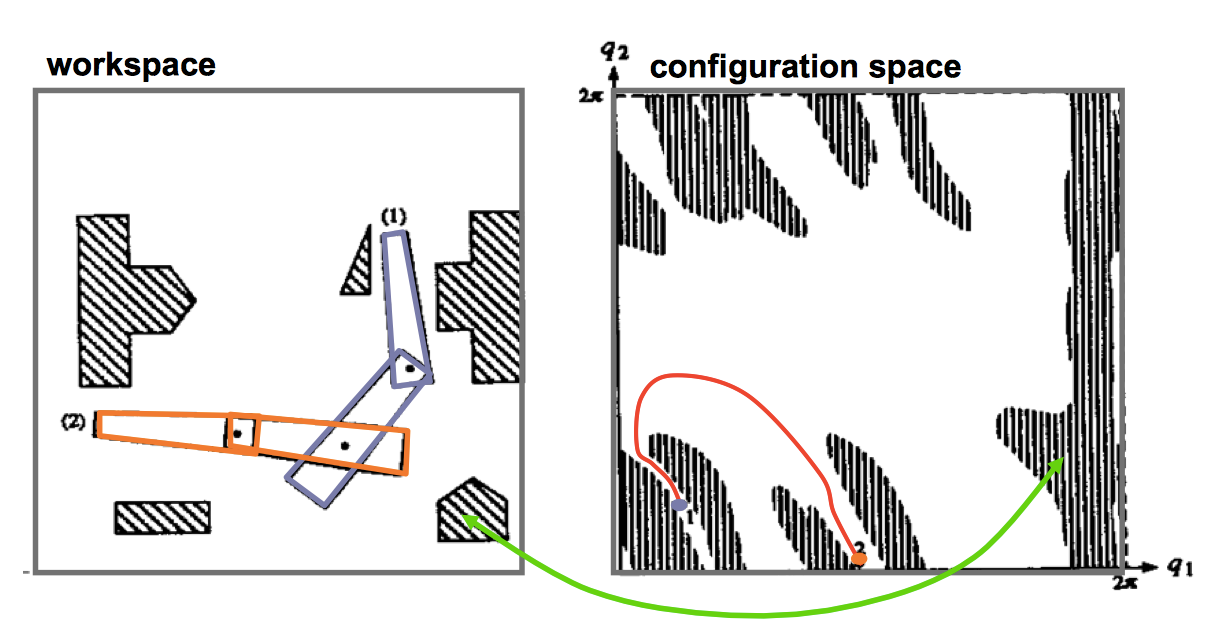
\includegraphics[width=0.8\textwidth]{configspacetrafo.png}
    \caption{Example from \cite{prmlec} for an indicator function in robotics. 
    		The given obstacles on the left are transformed 
		into occupied areas of the configuration space on the right.}
    \label{fig:awesome_image}
\end{figure*}

In the paper, the PRM algorithm is used to find trajectories for a robot arm, which avoid self collisions and collisions with obstacles in the environment.
Such trajectories can be expressed as functions describing the joint variables changing over time, that means as a curve in the configuration space with dimension equal to the number of degrees of freedom of the robot.
With this association, the trajectory finding problem becomes a path finding problem in the configuration space exactly of the form defined in the previous section.
The real obstacles transform into occupied areas in the configuration space. Those areas are given by the indicator function, which returns for a given vector of joint angles, if it is feasible or leads to a collision.


\subsection{Project Overview}

Like in the stated robotics example, in many cases the most costly operations of the PRM algorithm are the many evaluations of the indicator function \(I(q)\), 
which however can be done independently for every new \(q\).
Therefore the evaluation is implemented in a vectorized form as a function \((q_1, ... , q_P) \mapsto (I(q_1),...,I(q_P))\). 
The single indicator function computations are done in parallel on one or more graphics processing units (GPU).
The implementation is done with the programming interface CUDA \cite{cuda}, \cite{cuda2} by Nvidia.
In the robotics case, this means, the direct kinematics and collision calculations are made on the GPU in parallel for different joint angle configurations.
Although this will the only major application in the paper, the PRM solver and the configuration space are implemented separately to provide a flexible interface, as shown in figure \ref{interfacefig}. 
%As an example and for testing, additionally a simple 2D configuration space is provided, whose indicator function is read from a black-and-white image.

While the distribution of the indicator function to different CUDA threads is a first level of parallelization, 
a second level can be achieved by sampling and connecting several new nodes in parallel. 
This is more difficult, because all new nodes have to be connected 
and the graph data has to be updated on all processes. 
Different approaches have been implemented, with a description provided in chapter \ref{solver}.
Before that, chapter \ref{indicator} gives more details about the robotics indicator function.

\begin{figure*}
\begin{center} 
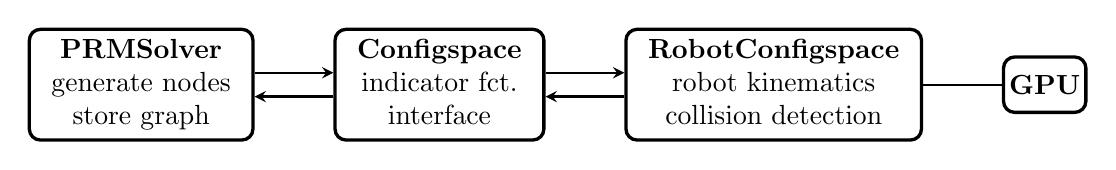
\begin{tikzpicture}[auto]%node distance=0.5cm and 1.8cm]
	\node[block] (prm) {
		\begin{tabular}{c}
		\textbf{PRMSolver}\\
		generate nodes\\
		store graph
		\end{tabular}
	};
	\node [block, right=of prm] (config) {
		\begin{tabular}{c}
		\textbf{Configspace}\\
		indicator fct. \\
		interface
		\end{tabular}
	};
	\node [block, right=of config] (robo) {
		\begin{tabular}{c}
		\textbf{RobotConfigspace}\\
		robot kinematics\\
		collision detection
		\end{tabular}
	};
	\node [block, right=of robo] (gpu) {\textbf{GPU}};
	
	\path[-stealth,thick, shift left=1.0ex]	(prm) edge (config) ;
	\path[-stealth,thick, shift left=1.0ex]	(config) edge  (prm) ;
	\path[-stealth,thick, shift left=1.0ex]	(config) edge (robo);
	\path[-stealth,thick, shift left=1.0ex]	(robo) edge  (config);
	\path[-,thick]					(robo) edge (gpu);
\end{tikzpicture}
\end{center}
\caption{Project structure. Probabilistic roadmap solver and configuration space implementation are separated.}\label{interfacefig}
\end{figure*}



%%%%%%%%%%%%%%%%%


\section{Implementation of an Indicator Function for Robot Arms}\label{indicator}

The probabilistic roadmap algorithm is applied  to create collision-free trajectories of a robot arm.
For a robot with given joint angles \(q_i\) one can calculate straightforward all positions and orientations  of the single parts of the robot.
For this, coordinate frames according to the Denavit-Hartenberg (DH) \cite{robodyn} convention are used.
The coordinate frames of reference of the single parts are described by transformation matrices 
$T_i \in \R^{4 \times 4}, i=1,...,d$, which transform points from the body frame of reference into the world frame of reference. They depend on the state $q=(q_1,...,q_d)^T$ of the robot and on the geometry of the joint angles given by the DH parameters of the robot. 

The geometry of the robot parts is defined by a set of convex polytopes, each of them belonging to one of the robot coordinate frames. Applying the corresponding transformation $T_i$, the vertices are transformed into the world frame. 
Environment obstacles are also defined by convex polytopes, given in the world frame.

Now the movement of the robot can be described by a curve $q(t) \in \R^d, t\in[0,1]$, in the configuration space. 
The movement is collision-free, if at no time, any two polytopes of the robot intersect with each other or with the environment after being transformed into the world frame.
To apply the probabilistic roadmap algorithm, we express this setting by the indicator function
\begin{equation}
	I(q)=
	\begin{cases}
		0,	& \text{ for no collision of any polytope pair} \\
		1,	& \text{ if at least one collision occurs }
	\end{cases}
	\; .
\end{equation}

The indicator function is implemented in a vectorized form in a CUDA kernel, which means that, given a set of states $q^1,..,q^M$, the indicator function is evaluated for each state by one CUDA thread. 
Therefore, the kinematics and collision algorithm are implemented as device code for the use in the CUDA kernel.

It has to be noted that the trajectories \(q(t)\), generated by the PRM algorithm, are piecewise linear and are therefore not differentiable at all points. 
Hence, before the use on a robot they have to be smoothed. 
This is not included in the project. 
The task is only to generate feasible trajectories to be possibly passed to an optimizer.

\subsection{Direct Kinematics}\label{dk}

The Denavit-Hartenberg convention is a method to describe the geometry of the joints of a robot, 
that is, how the transformations between the robot coordinate frames look like in dependency of its joint values $q_1,...,q_d$.
A robot consists of $d+1$ bodies each of which has a coordinate frame $B_i$ attached to the body, which is described by the transformation matrix $T_i$ to the world frame.
It is assumed that each joint is either rotational, that means a rotation around a fixed axis is performed, 
or prismatic, where a translation along an axis is performed.
These joints can now be defined through DH parameters $a_{i-1}, \alpha_{i-1}, d_i, \theta_i \in \R$, $i=1,...,d$, 
by setting up the transformations $T_{i-1,i}=T_{i-1}^{-1} T_{i}$ between two bodies as
\begin{equation}
	T_{i-1,i} = R_z(\theta_i) T_z(d_i) R_x(\alpha_{i-1}) R_x(a_{i-1})
\end{equation}
where $R_x, R_z$ are rotations aro\-und and $T_x, T_z$ are translations along the $x$ and $z$ axes.
With this and $T_0=I$, all transformations $T_i$ are determined.

One can show, that by an proper choice of the body frames, every robot with rotational or prismatic joints can be described by such a set of DH parameters, i.e. there exists a set of parameters, such that the above definition leads to the correct transformations for this robot.
For the exact calculations, see \cite{robodyn}.


\subsection{2D and 3D Geometry Library}

For the implementation of the kinematics and later the collision algorithm, a geometry library was written, based on the CUDA datatypes \texttt{float2} for 2D vectors and \texttt{float4} for 3D vectors.
To guarantee aligned access on the GPU, float4 is used instead of float3. 
Furthermore, as the precision of the geometric calculations is numerically not very critical, the usage of single precision instead of double precision did not cause problems.
The library contains host and device inline functions for common vector operations as shown in code \ref{code1}.
Operators like $+$ or $*$ are not overloaded to prevent unnecessary temporary variables.
Transformation matrices are implemented as float4 arrays with inline functions for common matrix operations. Again operators with temporaries were avoided, wherever possible.

\footnotesize
\begin{lstlisting}[language=C++, frame=single, float=*, 
	caption=Operator examples of the written float4 library.,
	label=code1
]
__host__ __device__ inline float4& operator += (float4& u, const float4& v);
__host__ __device__ inline float4& operator *=  (float4& u, const float f);
__host__ __device__ inline float4& add(const float4& u, const float4& v, float4& w);
\end{lstlisting}
\normalsize

\footnotesize
\begin{lstlisting}[language=C++, frame=single, float=*,
	caption=Class structure for a geomeric transformation matrix.,
	label=code2
]
class trafo4{
  public:
    float4 col[4];
    __host__ __device__ trafo4(){}
    __host__ __device__ trafo4(float a, float alpha, float q, float d);
    __host__ __device__ inline float4& apply(float4& u) const;
    __host__ __device__ inline float4& apply(const float4& u, float4& Tu) const;
    .
    .
}
\end{lstlisting}
\normalsize

\subsection{Polytopes}

To calculate the intersection between two convex polytopes, the Chung-Wang algorithm \cite{chung} is used. It only needs the polytope vertices 
and the data, which of them are connected by an edge. 
For this purpose, the adjacency matrix of the edge graph is stored in compressed row storage format.

\footnotesize
\begin{lstlisting}[language=C++, frame=single,
	caption=Storing polytopes in CRS format.,
	label=code3
]
struct polytope4{
    //vertices
    float4* vertices;	//length n
    int n; 	
    //edge adjacency matrix
    int* dsp;	//length n
    int* cnt;	//length n
    int* dest;	//length m
    int m;
};
\end{lstlisting}
\normalsize

This means, that for $i=0,...,n-1$ the vertices with indices \texttt{ dest[dsp[i]],...,dest[dsp[i]+cnt[i]-1] } are the ones connected to vertex $i$ by an edge.
The polytopes are given by the user as convex hull of a list of vertices. However, to determine the edge graph only from the vertices is a nontrivial task, which is done by Matlab using builtin high level functions.


\subsection{Chung-Wang Collision Algorithm}

To check if two polytopes collide an algorithm by Chung and Wang \cite{chung} is used here. It uses the separating vector theorem and tries to find a separating vector by an iterative search. Furthermore, a sub-algorithm determines in each iteration from the candidate history, if it is still theoretically possible to find a separating vector. 
If not, a collision is returned.
If on the other hand a separating vector is found, the algorithm returns no collision.
For a detailed description of the algorithm see \cite{chung} and \cite{ericson}, pp. 410-412.
The method is implemented as device code for the use in CUDA kernels.

In our application, the polytopes are mostly parts of the robot, which are given in the body frame of reference and have to be first transformed into world frame according to section \ref{dk}.
However, from the structure of the Chung-Wang algorithm follows, that only a small number of the polytope vertices are needed for the computations. 
Therefore, it would be rather wasteful to transform all vertices before passing them to the algorithm. 
To avoid this problem, all polytopes are passed in their body frames together with their transformations 
and the algorithm transforms a vertex, whenever it is needed in the calculations.
This is also the version proposed in \cite{chung}.

%\footnotesize
%\begin{lstlisting}[language=C++, frame=single, float=*]
%__host__ __device__ int separating_vector_algorithm(const polytope4& P, const polytope4& Q, const trafo4& tp, const trafo4& tq);
%\end{lstlisting}
%\normalsize

\subsection{Robot Kernel}

\footnotesize
\begin{lstlisting}[language=C++, frame=single, float=*,
	caption=Robot configuration space class structure.,
	label=code4
]
template<int ndof>
class RobotConfigspace : public Configspace<ndof>
{
public:
  RobotConfigspace(const Robot<ndof>* robot_,
                   const polytope *polys_,
                   const int* sys_,
                   const int N_,
                   const int *from_, const int *to_,
                   const int M_,
                   const float* mins_, const float* maxs_, const float dq_,
                   const int nbuf_);
  int init(const int ressource_rank=0, const int ressource_size=1);
  int indicator2(const float* qs, const float* qe, int *res, const int N, const int offset);
  .
  .
private:
  const Robot<ndof>* robot; //host object
  Robot<ndof>* robotdev;    //GPU object
  collision4::polytope4data* polydata;    //host object
  collision4::polytope4data* polydatadev; //GPU object
  collision4::polytope4data_restrict* polydatadev_restrict; //restricted pointers collection
  .
  .
}
\end{lstlisting}
\normalsize

%\footnotesize
%\begin{lstlisting}[language=C++, frame=single, float=*,
%	caption=GPU collision kernel for testing robot configurations.,
%	label=code5
%]
%__global__ void kernel_indicator2(const Robot<ndof>* robot,
%                                  const collision4::polytope4data* polydata,
%                                  const float* qs, int offsets,
%                                  const float* qe, int offsete,
%                                  int* res,
%                                  const int* testpos, const int* testnum,
%                                  int N, int numthreads);
%\end{lstlisting}
%\normalsize

\footnotesize
\begin{lstlisting}[language=C++, frame=single, float=*,
	caption=GPU collision kernel for testing robot configurations.,
	label=code5
]
__global__ void kernel_indicator2(const Robot<ndof>* __restrict__ robot,
                                  const collision4::polytope4data_restrict polydata,
                                  const float* __restrict__ qs, int offsets,
                                  const float* __restrict__ qe, int offsete,
                                  int* res,
                                  const int* __restrict__ testpos, const int* __restrict__ testnum,
                                  int N, int numthreads)
\end{lstlisting}
\normalsize


Code \ref{code4} exemplarily shows the class definition of the robot configuration space.
The geometry and robot data does not change during runtime
and is load\-ed once at the beginning and copied to the GPU by the 
\texttt{init}
function.
The indicator function gets as input a list of start and end points $q_{start}^j, q_{end}^j, j=0,...,N$ and checks now for each pair, if the indicator function is always 0 on the line in between.
\begin{equation}
	\mathrm{res[j]}=\begin{cases}
		%0	&\text{if $I(q)=0$ f.a. $q \in \left[q_{start}^j, q_{end}^j\right]_{\Delta q}$} \\
		0	&\text{if\ \ } \forall q \in \left[q_{start}^j, q_{end}^j\right]_{\Delta q} : I(q)=0 \\
		1	&\text{else}
	\end{cases}
\end{equation}
This computation is done by calling the kernel in Code \ref{code5}.
The start and end points are stored in structures of arrays defined by
\begin{equation}
\begin{aligned}
	q_{start}^j &\defgl (q_s^j , q_s^{j+N_{buf}} , ... , q_s^{j+(d-1)*N_{buf}})^T\\
	q_{end}^j &\defgl (q_e^j , q_e^{j+N_{buf}} , ... , q_e^{j+(d-1)*N_{buf}})^T
\end{aligned}
\end{equation}
As the PRM solver only needs to know, which start and end points can be connected by a line, the kernel delivers exactly this minimal necessary information. 
CPU and communication time is also saved by computing interpolating points directly on the GPU and not to exchange them.
Algorithms \ref{host} and \ref{kernel} show in pseudo code, how the work is split between host and device.

\begin{algorithm}\label{host}
	\KwData{$q_s$, $q_e$, N, $N_{buf}$}
	\KwResult{res}
	compute distances $d_j = \abs{q_{end}^j - q_{start}^j}$ \;
	$\mathrm{testnum[j]} = d_j/{\Delta q}$: number of threads for each line \;
	$\mathrm{testpos[j]} = \mathrm{thread\ displacements}$ \;
	reset res \;
	call kernel with $\sum_{j=0}^N \mathrm{testnum[j]}$ threads \;
	\caption{Host indicator function}
\end{algorithm}

\begin{algorithm}\label{kernel}
	\KwData{arrays $q_s$, $q_e$, testpos, testnum and threadindex}
	\KwResult{res}
	compute associated edge number $j$, defined by $testpos[j] \leq threadindex \le testpos[j]+testnum[j]$ \;
	$c = (\mathrm{threadindex - testpos[j]}) / (\mathrm{testnum[k]}-1) $ \;
	$q=c q_{start}^j + (1-c) q_{end}^j $ \;
	calculate robot kinematics $T_0(q), ..., T_d(q) $ \;
	$\mathrm{res\_tmp} = 0$ \;
	\For{all registered pairs pairs of polytopes $P, Q$}{
		$\mathrm{res\_tmp}=\mathrm{separating\_vector\_algorithm}(P, T_{i_P}, Q, T_{i_Q})$ \;
		\If{$\mathrm{res\_tmp} \neq 0$}{
			$\mathrm{res}[j]=\mathrm{res\_tmp}$ \;
			break \;
		}
	}
	\caption{Robot kernel: code for one thread}
\end{algorithm}

Furthermore, in order to overlap computations on the GPU and CPU, an asynchronous version of the indicator function was implemented. 
Here the host function is split into the part till the kernel launch and a function, which waits, until the kernel has finished and receives the result data.
This implementation also allows overlapping of multiple requests, for example two calls of the launch function and then the two corresponding waiting calls. 
With that, it is possible to use the full computation power of the GPU.

%\footnotesize
%\begin{lstlisting}[language=C++, frame=single, float=*,
%	caption=Asynchronous versions of indicator functions.,
%	label=code6
%]
%int indicator2_async(const float* qs, const float* qe, int *res, 
%                     const int N, const int offset, int &request);
%int indicator2_async_wait(int request);
%\end{lstlisting}
%\normalsize


%%%%%%%%%%%%%%%%%%%%%%%%

\section{The PRM Solver}\label{solver}

The solver builds in a first phase the roadmap graph from both the start and the end node, until the graph is connected.
It is always ensured that the graph consists of two connected components containing the start respectively the end node.
With this fact, it can be easily determined at each step, if the whole graph is now connected.

At the end, in a second phase of the algorithm, a shortest path from the start to the end node is searched by the Dijkstra algorithm.
It was observed, that this part of the algorithm needs a neglectable amount of time compared to building the graph.
Therefore, it is not parallelized here and the focus lies on the first phase.

\subsection{Storing the Graph}

Apart from the indicator function evaluation, the main problem in building the probabilistic roadmap is, 
that for each new node $q$ all possible neighbors have to be determined.
That is the set of all nodes $\tilde q$ of the graph, with $\norm{\tilde q - q} \le D$, with $D>0$ an ajustable algorithm parameter.
If no special order of the nodes is given, one has to calculate these norms for all nodes of the graph, which is rather time consuming.
Therefore, a special indexing is used. 
The nodes are stored in a vector, which is organized in blocks with fixed sizes. The blocks are referred to by ids which are stored in a map. See Code \ref{code7} for the data structures.

\footnotesize
\begin{lstlisting}[language=C++, frame=single, float=*,
	caption=Roadmap graph structure.,
	label=code7
]
struct block{
	int pos;	//! position of first vertex
	int num;	//! current number of vertices stored
	block* next; 	//! if num==blocksize -> pointer to next block
};

struct graph{
    std::map<int,block*> map; //map for accessing blocks
    std::vector<block> blocks;
    std::vector<float> qstorage; //length ndof*N
    int newblockpos;  //position of next new block
    int blocknum;     //number of used blocks
    .
    .
};
\end{lstlisting}
\normalsize

The key of a block is computed by the mapping
\begin{equation}
	key(q) = \left\lfloor \frac{q_1}{H} \right\rfloor
\end{equation}
such that $H>0$ becomes a parameter to adjust the grid density.
The parameter $H$ has to be chosen so large that enough nodes are stored in one block in order to have efficient memory accesses.
On the other hand, the smaller $H$ is, the less unnecessary computations have to be done for the neighborhood requests.
For illustration of the structure, the following pseudocode, algorithm \ref{keyalg}, shows the insertion of a node.

\begin{algorithm}\label{keyalg}
	\KwData{$q\in\R^d$}
	Compute key=key(q)\\ 
	\eIf{key exists in map}{
		block=map[key]\\ 
		\While{ block full }{
			block=block->next
		}
	}{
		insert new block at map[key]
	}
	Insert node into block
	\caption{Inserting a node}
\end{algorithm}

For getting the neighbors of a node $q$ it is then enough to look at the keys from $key(q_1-cD)$ to $key(q_1+cD)$. 
If $D=H$, then $c=1$ is possible.
The key mapping could be generalized by taking more components of $q$ into account or using kd-trees, see \cite{prm1}, p. 209, but that was not implemented.

\subsection{Parallelization Approaches}

The main parallelization is done with MPI. All processes store their own versions of the graph, which are held up to date between the processes.
It is assumed that every process has its own GPU.
The work of a single MPI process could be parallelized further with OpenMP, but this has not been pursued.
Instead, different approaches to distribute the work over several GPUs have been investigated.

\subsubsection*{Version 1} 

In the first approach, that has been evaluated, every process generates new nodes independently from each other.
Then the possible neighbors are determined and the connections which have to be tested.
The indicator function is called and returns the edge data.
After this, the graph must be synchronized between all processes, which needs an MPI all-to-all communication call.
As the graph building phase does not need the edge data, it is sufficient to exchange only the nodes and collect the edges at the end.

%\begin{figure}	
\begin{center}
\resizebox{\columnwidth}{!}{
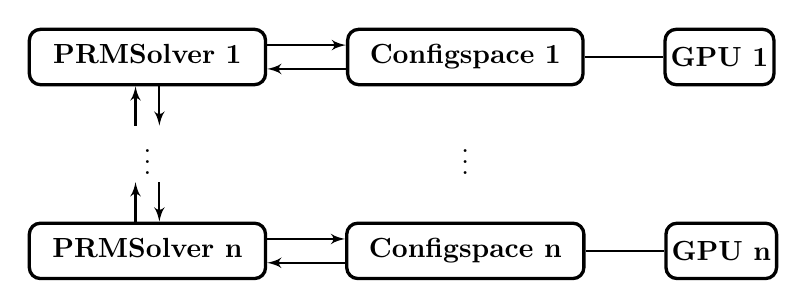
\begin{tikzpicture}[auto, node distance=0.5cm and 1.0cm]
	\node[block, minimum width=3cm] (prm) {
		\begin{tabular}{c}
		\textbf{PRMSolver 1}
		\end{tabular}
	};
	
	\node[frameless, below=of prm, minimum width=3cm] (space) {$\vdots$};
	
	\node[block, below=of space, minimum width=3cm] (prm2) {
		\begin{tabular}{c}
		\textbf{PRMSolver n}
		\end{tabular}
	};
	
	\node [block, right=of prm] (config) {
		\begin{tabular}{c}
		\textbf{Configspace 1}
		\end{tabular}
	};
	\node[frameless, below=of config] (space2) {$\vdots$};
	\node [block, below=of space2] (config2) {
		\begin{tabular}{c}
		\textbf{Configspace n}
		\end{tabular}
	};
	
	
	
	\node [block, right=of config] (gpu) {\textbf{GPU 1}};
	\node [block, right=of config2] (gpu2) {\textbf{GPU n}};
	
	
	\path[-latex',thick, shift left=1.0ex]	(prm) edge (config) 
								(config) edge (prm);
	\path[-,thick]					(config) edge (gpu);
	
	\path[-latex',thick, shift left=1.0ex]	(prm2) edge (config2) 
								(config2) edge (prm2) ;
	\path[-,thick]					(config2) edge (gpu2);
	
	
	\path[-latex',thick, shift left=1.0ex]	(prm) edge (space)
								(space) edge (prm)
								(prm2) edge (space)
								(space) edge (prm2) ;
	

\end{tikzpicture}
}
\end{center}
%\caption{First version of parallelization: distributed node generation.}
%\end{figure}	

\subsubsection*{Version 2}
The second approach uses the fact, that by synchronizing a random seed, 
different processes can produce the same sequence of random numbers independently from each other.
By using this property, every process can generate all new nodes and determine the connection data. 
Then the indicator function computation is split over their configuration space instances and the returned data shared afterwards with each other.
With this data, all graphs can be updated and it is guaranteed, that they grow exactly in the same way on each process.
The advantage of this version compared to the first one is, that less data has to be exchanged. 
Furthermore, in the first version it can occur, that the generated nodes can result in very different counts of neighbors and therefore uneven loads on the GPUs.
Here, the distribution of the computation amount over the GPUs can be chosen very flexible, without performance loss.


%\begin{figure*}	
\begin{center}
\resizebox{\columnwidth}{!}{
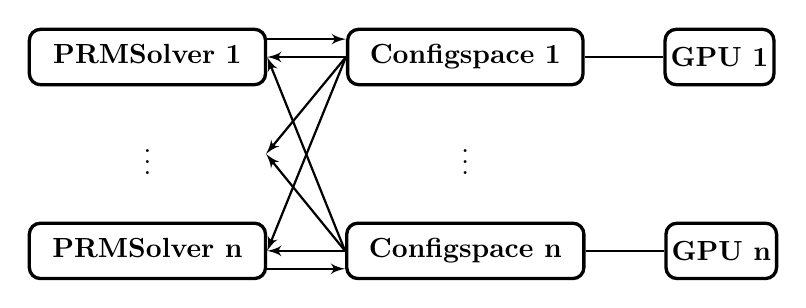
\begin{tikzpicture}[auto, node distance=0.5cm and 1.0cm]
	\node[block, minimum width=3cm] (prm) {
		\begin{tabular}{c}
		\textbf{PRMSolver 1}
		\end{tabular}
	};
	
	\node[frameless, below=of prm, minimum width=3cm] (space) {$\vdots$};
	
	\node[block, below=of space, minimum width=3cm] (prm2) {
		\begin{tabular}{c}
		\textbf{PRMSolver n}
		\end{tabular}
	};
	
	\node [block, right=of prm] (config) {
		\begin{tabular}{c}
		\textbf{Configspace 1}
		\end{tabular}
	};
	\node[frameless, below=of config] (space2) {$\vdots$};
	\node [block, below=of space2] (config2) {
		\begin{tabular}{c}
		\textbf{Configspace n}
		\end{tabular}
	};
	
	
	
	\node [block, right=of config] (gpu) {\textbf{GPU 1}};
	\node [block, right=of config2] (gpu2) {\textbf{GPU n}};
	
	
	\path[-latex',thick, shift left=1.5ex]	(prm) edge (config) ;
	\path[-,thick]					(config) edge (gpu);
	
	\path[-latex',thick, shift right=1.5ex]	(prm2) edge (config2) ;
	\path[-,thick]					(config2) edge (gpu2);
	
	
	\path[-latex',thick]				(config.west) edge  (prm.east) 
								(config.west) edge (space.east)
								(config.west) edge (prm2.east)
								(config2.west) edge  (prm.east) 
								(config2.west) edge (space.east)
								(config2.west) edge (prm2.east);

\end{tikzpicture}
}
\end{center}
%\caption{Second version of parallelization: redundant node generation. }
%\end{figure*}

\begin{figure}
\begin{center}
\resizebox{\columnwidth}{!}{
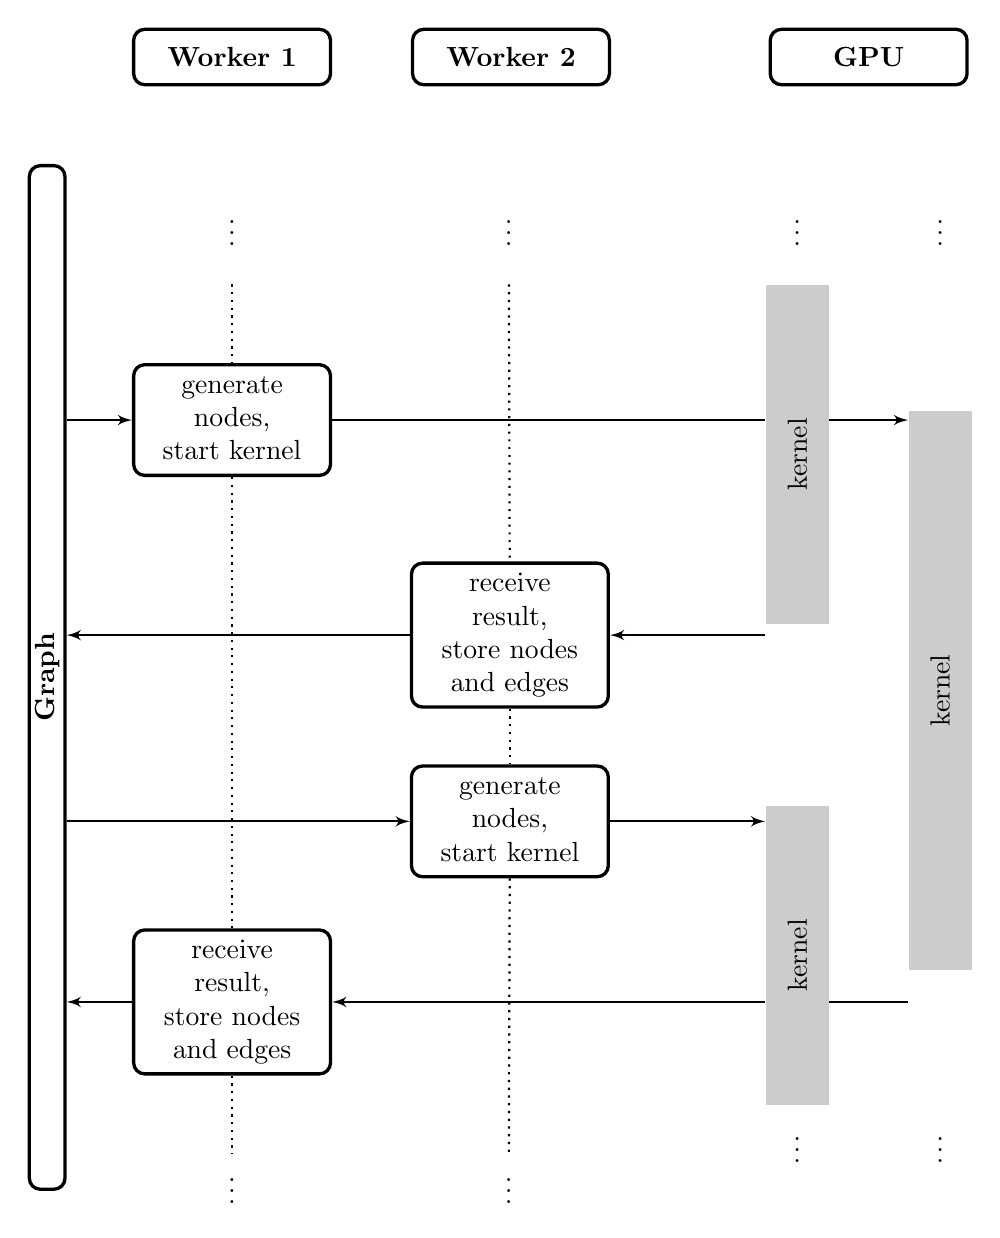
\begin{tikzpicture}
	\tikzset{mywidth/.style={minimum width=2.5cm},};
	\node[block, mywidth] (l1) {\textbf{Worker 1}};
	\node[frameless, mywidth, below=of l1, minimum height=1.5cm] (l2) {$\vdots$};
	\node[block, mywidth, below=of l2] (l3) 	{\begin{tabular}{c}
										generate\\ nodes, \\
										start kernel
									\end{tabular}};
	\node[frameless, mywidth, below=of l3, minimum height=2cm] (l6) {};
	\node[frameless, mywidth, below=of l6] (l7) {};
	\node[block, mywidth, below=of l7] (l11)	{\begin{tabular}{c}
										receive\\ result, \\
										store nodes \\ 
										and edges
									\end{tabular}};
	\node[frameless, mywidth, below=of l11] (l12) {$\vdots$};
	
	
	\node[block, mywidth, right=of l1] (r1) {\textbf{Worker 2}};
	\node[frameless, mywidth, right=of l2, minimum height=1.5cm] (r2) {$\vdots$};
	\node[frameless, mywidth, right=of l3] (r3) {};
	\node[block, mywidth, right=of l6] (r6)	{\begin{tabular}{c}
										receive\\ result, \\
										store nodes \\
										and edges
									\end{tabular}};
	\node[block, mywidth, right=of l7] (r7) 	{\begin{tabular}{c}
										generate\\ nodes, \\
										start kernel
									\end{tabular}};
	\node[frameless, mywidth, right=of l12] (r12) {$\vdots$};
	
	\node[frameless, left=of l1] (g1) {};
	\node[block, below=of g1, minimum height=13cm] (graph) {\rotatebox{90}{\textbf{Graph}}};
	
	
	%gpu column
	\tikzset{gpuwidth/.style={minimum width=0.8cm},};
	
	\node[block, right=2cm of r1, minimum width=2.5cm] {\textbf{GPU}};
	\node[frameless, right=2cm of r2, gpuwidth] (topa) {$\vdots$};
	\node[frameless, right=of topa, gpuwidth] (topb) {$\vdots$};
	\node[block2, below=0.4cm of topa, gpuwidth, minimum height=4.3cm] (stream1a) {\rotatebox{90}{kernel}};
	\node[block2, below=2.3cm of stream1a, gpuwidth, minimum height=3.8cm] (stream1b) {\rotatebox{90}{kernel}};
	\node[frameless, below=0.1cm of stream1b, gpuwidth] (bota) {$\vdots$};
	
	\node[block2, below=2.0cm of topb, gpuwidth, minimum height=7.1cm] (stream2) {\rotatebox{90}{kernel}};
	\node[frameless, right=of bota, gpuwidth] (botb) {$\vdots$};
	
	
	
	%EDGES
	
	\path[-latex',thick]	(graph.east |- l3.west) edge (l3.west)
					(l11.west) edge (graph.east |- l11.west);
	\path[-latex',thick]	(graph.east |- r7.west) edge (r7.west)
					(r6.west) edge (graph.east |- r6.west);
	\path[dotted,thick]	(l2) edge (l3)
					(l3) edge (l11)
					(l11) edge (l12)
					(r2) edge (r6)
					(r6) edge (r7)
					(r7) edge (r12);
	
	\path[-latex',thick]	(r6.east -| stream1b.west) edge (r6.east);
	\path[-latex',thick]	(r7.east) edge (r7.east -| stream1b.west);
	
	\path[-,thick]		(l3.east) edge (l3.east -| stream1a.west);
	\path[-latex',thick]	(stream1a.east |- l3.east) edge (l3.east -| stream2.west);
	\path[latex'-,thick]		(l11.east) edge (l11.east -| stream1b.west);
	\path[-,thick]		(stream1b.east |- l11.east) edge (l11.east -| stream2.west);
	
	
\end{tikzpicture}
}
\end{center}
\caption{Structure of asynchronous kernel launches.}\label{fig:v3}
\end{figure}

\subsubsection*{Version 3}

The third version includes a further optimization by using the asynchronous version of the indicator function.
Here, every process runs two workers overlapped,
between which the node generation and GPU requests are split up.
Figure \ref{fig:v3} shows the detailed work flow.
%In the time, when the first worker has generated his indicator function request, launched the kernel and now is waiting until it has finished, the second worker updates the graph and sends his new request, and the other way round.
With this, it is possible, that the computational ressources of the GPU are fully used, and overlapped with the communication. 

\section{Results}

\begin{figure}%{r}{0.5\textwidth}
	\centering
	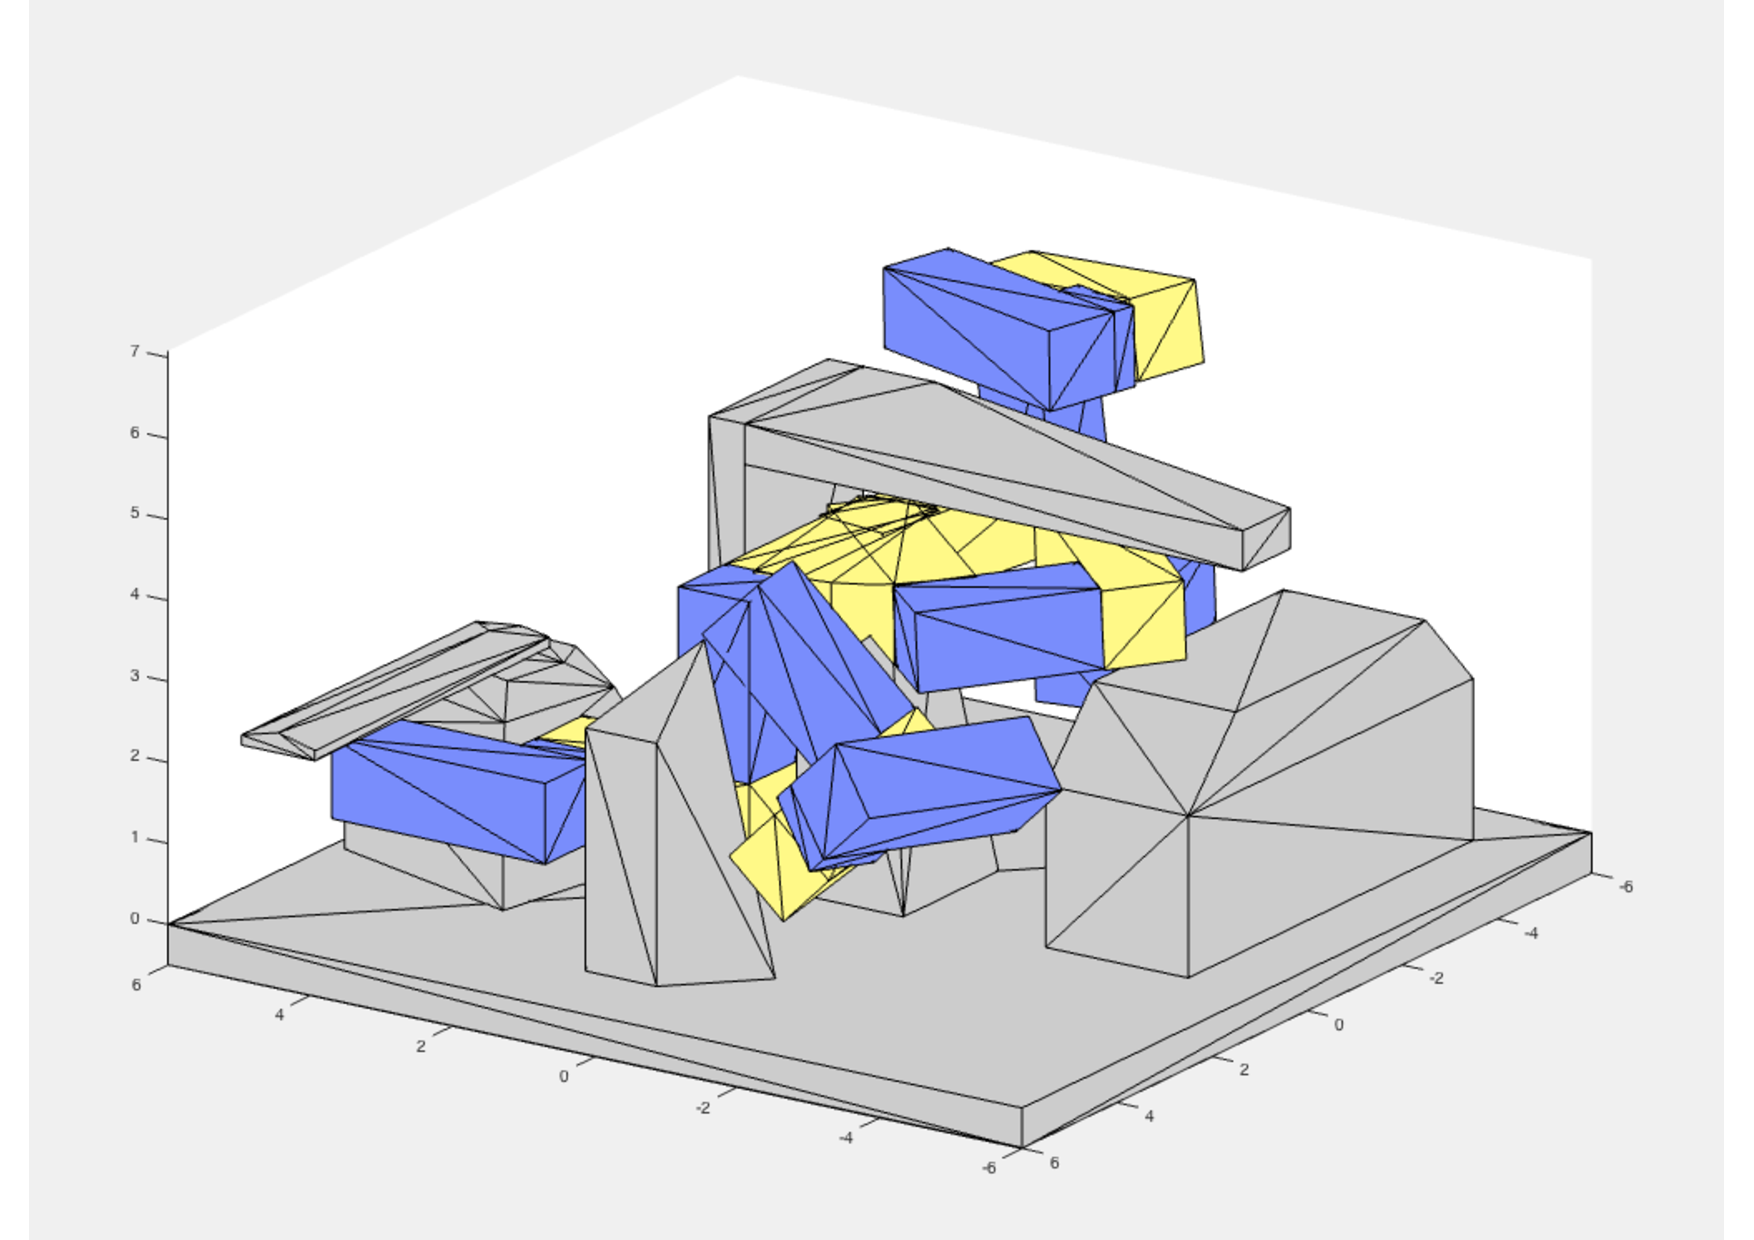
\includegraphics[width=0.5\textwidth]{robotsolution2_5.pdf}
	\caption{PRM generated collision-free movement for a 4-axis robot}\label{robotpic}
\end{figure}

Benchmark runs have been performed for a realistic scenario with a robot with four joints, shown in figure \ref{robotpic}.
This scenario is difficult because of the small path to be passed in the middle of the domain in figure \ref{robotpic}.
For creating and plotting the environment and the resulting trajectories, Matlab functions were written.
Because of the dependency on random numbers, the execution times differ for different runs.
Therefore, 10 runs were made for each version and number of processes.
However, the different versions lead to a different average amount of GPU threads needed.
Hence, to be able to better compare how the benchmarks scale, the time per number of GPU threads is used as a quantity.
Table 1 shows the results.

\begin{table}
\caption{Timing results for the parallelization versions from chapter \ref{solver} on a cluster node with 2x Intel Xeon Eight-Core CPU E5-2650 0 @ 2.00GHz and 4x Tesla K20m.}\label{resulttable}
\centering

\begin{tabular}{ c  c  r  r  r }

\hline
version	&  processes/	& time		& GPU 		& time per $10^6$  \\ 
		& GPUs		& (ms)		& threads		& threads (ms) \\ 
\hline
		& 1			& 6864		& 6171525	& 1070	\\ 
1		& 2			& 1580		& 4489213	& 342	\\ 
		& 4			& 869		& 5853763	& 149	\\ 
\hline
		& 1			& 2136		& 6933768	& 337	\\ 
2		& 2			& 1778		& 6933768	& 290	\\ 
		& 4			& 1677		& 6933768	& 279	\\ 
\hline
		& 1			& 2492		& 19096275	& 130	\\ 
3		& 2			& 1345		& 19096275	& 72		\\ 
		& 4			& 942		& 19096275	& 52		\\ 
\hline
\hline
version	&  CPU		& time		& indicator 	& time per $10^6$  \\ 
		& threads		& (ms)		& evaluations	& evals. (ms) \\
		
\hline
3		& 4			& 32730		& 10038198	& 3281	\\ 
 (CPU	& 8			& 17676		& 10038198	& 1785	\\ 
only)		& 16			& 9936		& 10038198	& 1012	\\ 
\hline

\end{tabular}
\end{table}


As the indicator function has also been implemented on the CPU, all versions could be run without GPU.
The timing results for the last one are shown in the last section of table \ref{resulttable}.
One can see an improvement of up to a factor around 10 between the CPU and GPU benchmarks (based on version 3).
However, the robot code is not especially optimized for the CPU version, as the GPU kernel has been rewritten with an for loop
reusing all device functions for collision detection.
The GPU performance significantly improves from version 1 to 3.
The code is available on Github, \cite{githubcode}.


%%%%%%%%%%%%%%%%%%%%%%%%

\begin{thebibliography}{}%{999}
	\bibitem{prmlec} D. Burschka, Lecture Robot Motion Planning, \url{http://robvis01.informatik.tu-muenchen.de/courses/wegtraj/index.html}
	\bibitem{prm1} H. Choset, K. Lynch, S. Hutchinson, G. Kantor, W. Burgard, L. Kavraki and S. Thrun, Principles of Robot Motion: Theory, Algorithms, and Implementation, MIT Press 2005
	\bibitem{prm2} S. M. LaValle, Planning Algorithms, Cambridge University Press 2006
	\bibitem{robodyn} T. Buschmann, Skript zur Vorlesung: Roboterdynamik SS14, Lehrstuhl f�r Angewandte Mechanik, TU M�nchen 2014
	\bibitem{chung} K. Chung, Wenping Wang, Quick Collision Detection of Polytopes in Virtual Environments, Proceedings of the ACM Symposium on Virtual Reality Software and Technology (VRST 96), Mark Green (ed.) 1996
	\bibitem{ericson} C. Ericson, Real-Time Collision Detection, MK 2005
	\bibitem{cuda} Nvidia Corporation, Cuda Programming Guide, 2015, \url{http://docs.nvidia.com/cuda/pdf/CUDA_C_Programming_Guide.pdf}
	\bibitem{cuda2} D. B. Kirk, W. W. Hwu, Programming Massively Parallel Processors, MK 2010
	\bibitem{c++} Pitt-Francis, Guide to Scientific Computing in C++, Springer 2012
	\bibitem{mpi} W. Gropp, Using MPI: Portable Parallel Programming with the Message-Passing Interface, MIT Press 2014
	\bibitem{githubcode} M. Demmeler, Github Repository GPUPRM, \url{https://github.com/demmeler/GPUPRM}
\end{thebibliography}

\end{document}

















